%% Copernicus Publications Manuscript Preparation Template for LaTeX Submissions
%% ---------------------------------
%% This template should be used for copernicus.cls
%% The class file and some style files are bundled in the Copernicus Latex Package, which can be downloaded from the different journal webpages.
%% For further assistance ,please contact Copernicus Publications at: production@copernicus.org
%% https://publications.copernicus.org/for_authors/manuscript_preparation.html


%% Please use the following documentclass and journal abbreviations for preprints and final revised papers.

%% 2-column papers and preprints
\documentclass[acp, manuscript]{copernicus}

%% Journal abbreviations (please use the same for preprints and final revised papers)


% Advances in Geosciences (adgeo)
% Advances in Radio Science (ars)
% Advances in Science and Research (asr)
% Advances in Statistical Climatology, Meteorology and Oceanography (ascmo)
% Annales Geophysicae (angeo)
% Archives Animal Breeding (aab)
% Atmospheric Chemistry and Physics (acp)
% Atmospheric Measurement Techniques (amt)
% Biogeosciences (bg)
% Climate of the Past (cp)
% DEUQUA Special Publications (deuquasp)
% Drinking Water Engineering and Science (dwes)
% Earth Surface Dynamics (esurf)
% Earth System Dynamics (esd)
% Earth System Science Data (essd)
% E&G Quaternary Science Journal (egqsj)
% EGUsphere (egusphere) | This is only for EGUsphere preprints submitted without relation to an EGU journal.
% European Journal of Mineralogy (ejm)
% Fossil Record (fr)
% Geochronology (gchron)
% Geographica Helvetica (gh)
% Geoscience Communication (gc)
% Geoscientific Instrumentation, Methods and Data Systems (gi)
% Geoscientific Model Development (gmd)
% History of Geo- and Space Sciences (hgss)
% Hydrology and Earth System Sciences (hess)
% Journal of Bone and Joint Infection (jbji)
% Journal of Micropalaeontology (jm)
% Journal of Sensors and Sensor Systems (jsss)
% Magnetic Resonance (mr)
% Mechanical Sciences (ms)
% Natural Hazards and Earth System Sciences (nhess)
% Nonlinear Processes in Geophysics (npg)
% Ocean Science (os)
% Polarforschung - Journal of the German Society for Polar Research (polf)
% Primate Biology (pb)
% Proceedings of the International Association of Hydrological Sciences (piahs)
% Safety of Nuclear Waste Disposal (sand)
% Scientific Drilling (sd)
% SOIL (soil)
% Solid Earth (se)
% The Cryosphere (tc)
% Weather and Climate Dynamics (wcd)
% Web Ecology (we)
% Wind Energy Science (wes)


%% \usepackage commands included in the copernicus.cls:
%\usepackage[german, english]{babel}
%\usepackage{tabularx}
%\usepackage{cancel}
%\usepackage{multirow}
%\usepackage{supertabular}
%\usepackage{algorithmic}
%\usepackage{algorithm}
%\usepackage{amsthm}
%\usepackage{float}
%\usepackage{subfig}
%\usepackage{rotating}
\usepackage{bibentry}

\usepackage[acronym]{glossaries}
% \makeglossaries
\newacronym{abi}{ABI}{Advanced Baseline Imager}
\newacronym{amv}{AMV}{Atmospheric Motion Vector}
\newacronym{boa}{BoA}{Bottom-of-Atmosphere}
\newacronym{bt}{BT}{Brightness Temperature}
\newacronym{cape}{CAPE}{Convective Available Potential Energy}
\newacronym{cc4cl}{CC4CL}{Community Cloud Retrieval for Climate}
\newacronym{cci}{CCI}{Climate Change Initiative}
\newacronym{ccn}{CCN}{Cloud Condensation Nuclei}
\newacronym{ceres}{CERES}{Clouds and the Earth's Radiant Energy System}
\newacronym{cin}{CIN}{Convective Inhibition}
\newacronym{conus}{CONUS}{Continental United States}
\newacronym{cpr}{CPR}{Cloud Profiling Radar}
\newacronym{cre}{CRE}{Cloud Radiative Effect}
\newacronym{cth}{CTH}{Cloud Top Height}
\newacronym{ctt}{CTT}{Cloud Top Temperature}
\newacronym{cb}{Cb}{Cumulonimbus}
\newacronym[% options to override defaults
    shortplural={DCCs},
    longplural={Deep Convective Clouds}
    ]{dcc}{DCC}{Deep Convective Cloud}
\newacronym{dis}{DIS}{Deep Inverse Search}
\newacronym{dualtvl1}{Dual TV-L\textsuperscript{1}}{Dual Total Variation Regularisation \& Robust L\textsuperscript{1} Norm}
\newacronym{ebaf}{EBAF}{Energy Balanced and Filled}
\newacronym{esa}{ESA}{European Space Agency}
\newacronym{eumetsat}{EUMETSAT}{European Organisation for the Exploitation of Meteorological Satellites}
\newacronym{far}{FAR}{False Alarm Rate}
\newacronym{fat}{FAT}{Fixed Anvil Temperature}
\newacronym{gcm}{GCM}{Global Climate Model}
\newacronym{ghg}{GHG}{Greenhouse Gas}
\newacronym{glm}{GLM}{Geostationary Lightning Mapper}
\newacronym{goes}{GOES}{Geostationary Operational Environment Satellite}
\newacronym{inp}{INP}{Ice Nucleating Particle}
\newacronym{ir}{IR}{Infrared}
\newacronym{itcz}{ITCZ}{Inter-Tropical Convergence Zone}
\newacronym{jaxa}{JAXA}{Japan Aerospace Exploration Agency}
\newacronym{jma}{JMA}{Japanese Meteorological Agency}
\newacronym{lcl}{LCL}{Lifted Condensation Level}
\newacronym{lfc}{LFC}{Level of Free Convection}
\newacronym{lnb}{LNB}{Level of Neutral Buoyancy}
\newacronym{lw}{LW}{Longwave}
\newacronym{lwc}{LWC}{Liquid Water Content}
\newacronym{mcmip}{MCMIP}{Multi-channel Cloud and Moisture Imagery Product}
\newacronym{mcs}{MCS}{Mesoscale Convective System}
\newacronym{mse}{MSE}{Mean Square Error}
\newacronym{msg}{MSG}{Meteosat Second Generation}
\newacronym{nexrad}{NEXRAD}{Next Generation (Weather) Radar}
\newacronym{ngp}{NGP}{Northern Great Plains}
\newacronym{nir}{NIR}{Near Infrared}
\newacronym{noaa}{NOAA}{National Oceanic and Atmospheric Administration}
\newacronym{od}{OD}{Optical Depth}
\newacronym{pbl}{PBL}{Planetary Boundary Layer}
\newacronym{pca}{PCA}{Principle Component Analysis}
\newacronym{phat}{PHAT}{Proportionately Higher Anvil Temperature}
\newacronym{pod}{POD}{Probability of Detection}
\newacronym{rgb}{RGB}{Red, Green, Blue}
\newacronym{re}{r\textsubscript{e}}{Effective Radius}
\newacronym{seviri}{SEVIRI}{Spinning Enhanced Visible Infra-Red Imager}
\newacronym{sw}{SW}{Shortwave}
\newacronym{swd}{SWD}{Split Window Difference}
\newacronym{toa}{ToA}{Top-of-Atmosphere}
\newacronym{usa}{USA}{United States of America}
\newacronym{utc}{UTC}{Universal Co-ordinated Time}
\newacronym{wsr88d}{WSR-88D}{Weather Surveillance Radar, 1988, Doppler}
\newacronym{wv}{WV}{Water Vapour}
\newacronym{wvd}{WVD}{Water Vapour Difference}

\renewcommand{\thefigure}{S\arabic{figure}}


\begin{document}

\begin{figure*}[p]
    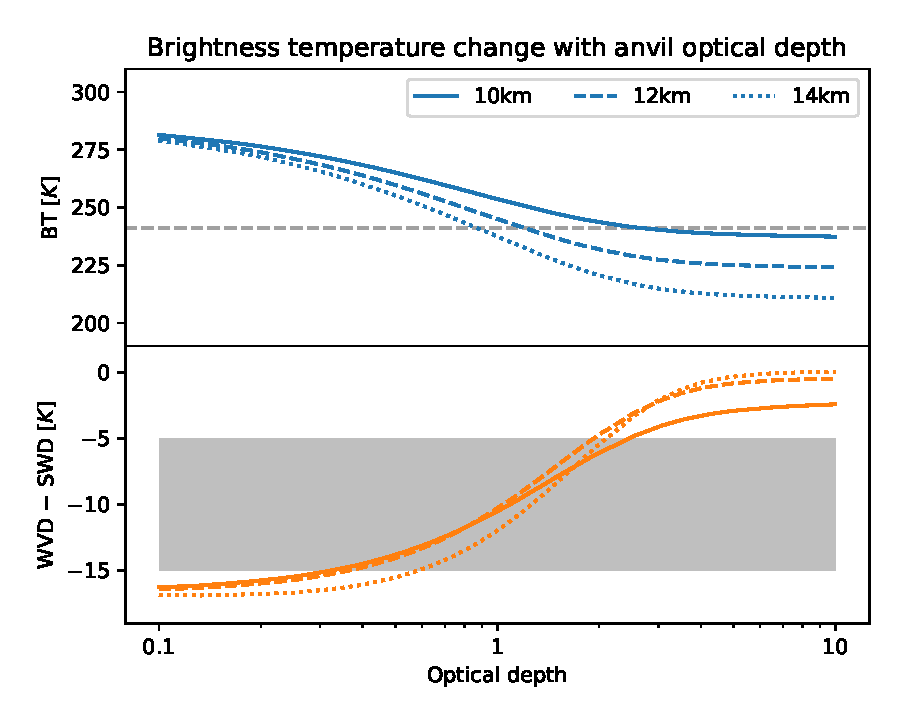
\includegraphics[width=12cm]{figures/fig_S01.pdf}
    \caption{
    Simulated sensitivity of the \acrshort{seviri} 10.8\,\unit{\mu m} \acrshort{bt} (top) and \acrshort{wvd} minus \acrshort{swd} (bottom) to anvil clouds of varying optical thickness (at 550\,\unit{n m}) at heights of 10, 12 and 14\,\unit{km}. The LibRadTran model was used to estimate the observed radiances, and all simulations used ice clouds with cloud top particle effective radius of 20\,\unit{\mu m}. The grey dashed line shows the 241\,\unit{K} \acrshort{bt}, which, although commonly used as a threshold for anvil detection in satellite imagery, shows large sensitivity of the minimum optical thickness detected with the height of the anvil cloud. The grey region in the lower plot shows the range of temperatures in which the edge of the anvil is detected, as described in \citet{jones_semilagrangian_2023}. Similar sensitivity is found for all three cloud heights, with the optical depths of around 1--1.5 seen in the middle of the hysteresis region. The median minimum retrieved optical depth of all tracked anvils in our dataset is found to be 1.45, although this value is biased high by the inability to retrieve optical depth accurately at night-time.
    }
    \label{fig:S_anvil_sensitivity}
\end{figure*}

\begin{figure*}[p]
    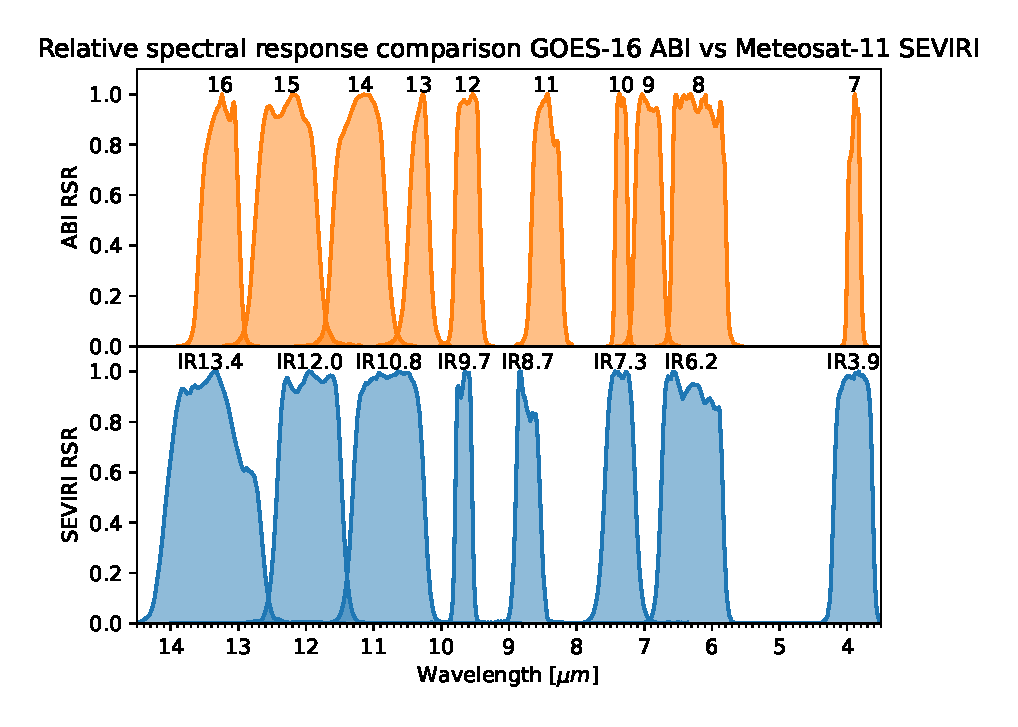
\includegraphics[width=12cm]{figures/fig_S02.pdf}
    \caption{
    Comparison of the relative spectral response (RSR) functions for the \acrshort{goes}-16 \acrshort{abi} and Meteosat-11 \acrshort{seviri} thermal \acrshort{ir} channels. The \acrshort{lw} window channels on \acrshort{abi} (channels 13 and 15) have a wider spacing than those of \acrshort{seviri} (channels IR10.8 and IR12.0). This wider spacing allows \acrshort{abi} to be more sensitive to the emissivity difference of ice clouds at wavelengths between 10 and 12\,\unit{mu m}, and so it is better able to detect thin cirrus clouds.}
    \label{fig:S_abi_seviri_rsr}
\end{figure*}

\begin{figure*}[p]
    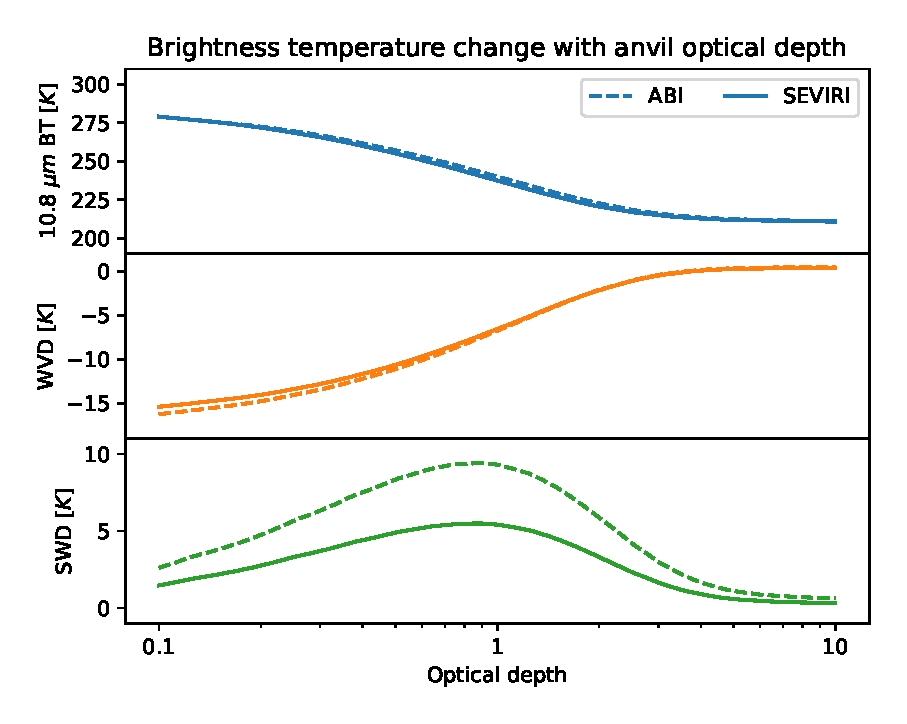
\includegraphics[width=12cm]{figures/fig_S03.pdf}
    \caption{
    Comparison of the sensitivities of \acrshort{abi} (dashed lines) and \acrshort{seviri} (solid lines) to anvil clouds of different cloud optical thicknesses (at 550\,\unit{n m}), using the LibRadTran simulation of an anvil at 14\,\unit{km} as used in fig.~\ref{fig:S_anvil_sensitivity}. The 10.8\,\unit{\mu m} \acrshort{bt} (top panel) and \acrshort{wvd} (middle panel) show very similar values for both instruments. The simulations of the \acrshort{swd} (bottom panel) show that \acrshort{seviri} is only about half as sensitive as \acrshort{abi} to thin ice clouds.
    }
    \label{fig:S_abi_seviri_anvil_sensitivty}
\end{figure*}

\begin{figure*}[p]
    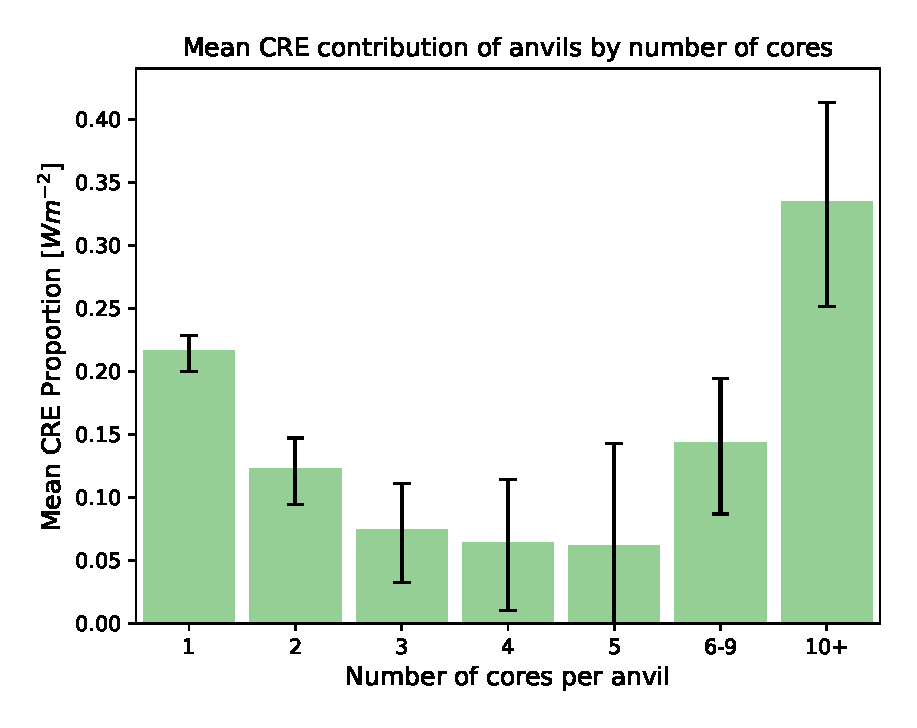
\includegraphics[width=12cm]{figures/fig_S04.pdf}
    \caption{
    The contribution to the net CRE for anvils with differing numbers of cores, which is defined as the sum of the absolute CRE multiplied by anvil area for all anvils with that number of cores, divided by the total for all anvils. Due to the large variance and magnitude of the CRE of isolated DCCs, they have a large impact on the net CRE balance despite their small area. 
    }
    \label{fig:S_contribution_to_net_cre}
\end{figure*}

\bibliographystyle{copernicus}
\nobibliography{bibliography.bib}

\end{document}